% @author Benjamin Schröder
%
\chapter{Grundlagen}
In diesem Kapitel werden einige grundlegende Konzepte behandelt, welche zum Verständnis dieser Arbeit beitragen. Zunächst wird
erklärt, was genau unter dem Begriff der prozeduralen Generierung zu verstehen ist, woraufhin einige der fundamentalen Verfahren
vorgestellt werden.

\section{Prozedurale Generierung}
Prozedurale Generierung, oft auch \gls{ac:pcg}, beschreibt eine Menge von Verfahren zum
algorithmischen Erstellen von Inhalten ("Content"). Dabei handelt es sich meist um Verfahren, die automatisch Texturen
oder verschiedene Gebilde im Kontext von Videospielen erzeugen können, so z.B. Landschaften, Flüsse, Straßennetze,
Städte oder Höhlenstrukturen. \cite{14_carli_et_al} Auch Musik kann durch solche Verfahren generiert werden
\cite{28_ramanto_maulidevi}, was für diese Arbeit allerdings weniger relevant ist.

Diese Definition ist absichtlich etwas allgemeiner gehalten, da das Aufstellen einer spezifischeren Definition nicht
besonders trivial ist. Das Konzept von \gls{ac:pcg} wurde bereits aus vielen veschiedenen Blickwinkeln beleuchtet und ist für verschiedene
Personen von unterschiedlicher Bedeutung. So hat z.B. ein Game Designer eine etwas andere Perspektive als ein Wissenschaftler, der
sich lediglich in der Theorie mit der Thematik beschäftigt. Verschiedene Definitionen unterscheiden sich in Bezug auf
Zufälligkeit, die Bedeutung von "Content", oder darin, ob und in welchem Umfang menschliche Intervenierung eine Rolle in einem
Verfahren spielen darf. Mit diesem Problem haben sich Togelius et al. \cite{9_togelius_et_al} bereits ausführlich befasst, weshalb dies hier
nicht weiter thematisiert werden soll. Für diese Arbeit soll die oben genannte Definition ausreichen.

\section{Verwendung von PCG}
% evtl. weglassen?
Da die Entwicklung von Videospielen aufgrund der großen Anzahl an benötigten Inhalten sehr schnell sehr aufwändig werden
kann, findet \gls{ac:pcg} vor allem in dieser Industrie einen großen Nutzen. Gerade das Erstellen von immersiven Welten erfordert eine Vielzahl
von verschiedensten detaillierten Modellen und kann manuell nur mit sehr großem Arbeitsaufwand umgesetzt werden. Das Automatisieren der
Generierung von Inhalten kann den Entwicklerstudios hier eine bedeutende Menge an Zeit und Kosten sparen, die dann an anderen
Stellen eingesetzt werden können. In vielen Fällen kann sogar Speicherplatz gespart werden, indem die Generierung der Inhalte
zur Laufzeit stattfindet.

\gls{ac:pcg} hat bereits in vielen bekannten Videospielen Verwendung gefunden. Schon im Jahr 1980 wurde %rogue

TODO: Aufzählen von Spielen mit PCG Algorithmen

\section{Perlin Noise}
Ein fundamentales Konzept im Bereich von \gls{ac:pcg} ist das Verwenden von Rauschfunktionen, oder auch \textit{Noise}.
Der wohl bekannteste Vertreter dieses Konzepts ist das 1985 von Ken Perlin entwickelte \cite{16_perlin} und 2002 verbesserte \cite{18_perlin}
\textit{Perlin Noise}, welches seit dessen Veröffentlichung nicht mehr aus der Welt der Computergrafik wegzudenken ist. Mithilfe von
Perlin Noise können eine Reihe von Zufallswerten erzeugt werden. Hierbei sind sich nah beieinander liegende Werte stets sehr ähnlich und es
gibt keine starken Ausschläge, weshalb der entstehende Verlauf sehr organisch wirkt. Aufgrund von dieser Eigenschaft eignet sich Perlin Noise
perfekt zum Erzeugen von natürlichen Strukturen wie z.B. Hügellandschaften oder Inselgruppen. Generell ist der erzeugte Kurvenverlauf vielseitig
einsetzbar und findet somit in vielen verschiedenen Anwendungen einen Nutzen, darunter auch im Bereich der Animation. \cite{17_lagae_et_al}

TODO: Einfügen von Vergleich zwischen Random Noise und Perlin Noise

Neben der vielseitigen Einsetzbarkeit von Perlin Noise gibt es außerdem den Vorteil, dass dieses Verfahren sehr günstig sowohl in Bezug auf
die Berechnungszeit als auch in Bezug auf die Speicherverwendung ist. Einzelne Punkte im Verlauf lassen sich unabhängig voneinander berechnen,
wodurch sich der Berechnungsprozess wunderbar parallelisieren lässt. Dies wird mit der immer weiter voranschreitenden Entwicklung von
Grafikkarten und Prozessoren auch zu einem immer größeren Vorteil. \cite{17_lagae_et_al}

Perlin Noise kann für eine beliebige Anzahl an Dimensionen berechnet werden. Dazu wird der n-dimensionale Raum in eine reguläre gitterartige
Struktur aufgespalten. Die Punkte auf dem Gitter sind dabei all jene, die an ausschließlich ganzzahligen Koordinaten liegen. Im zweidimensionalen
Raum wäre dies also die Menge an Punkten \(\{(x, y) \ \| \ x, y \in \mathbb{N}\}\). Alle anderen Punkte im Raum befinden sich dann jeweils innerhalb
einer der von den Gitterpunkten aufgespannten Zellen.

\begin{figure}[h]
    \centering
    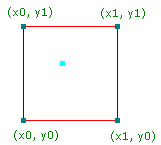
\includegraphics[height=\imgHeight]{images/noise_cell.png}
    \caption{Beispiel einer Gitterzelle im 2D}
    \label{fig:noise_cell}
\end{figure}

Jeder der Gitterpunkte bekommt außerdem einen pseudozufälligen Gradienten (Richtungsvektor der Länge 1) zugeordnet.

\begin{figure}[h]
    \centering
    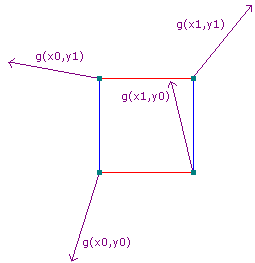
\includegraphics[height=\imgHeight]{images/noise_gradient.png}
    \caption{Pseudozufällige Gradienten für die Eckpunkte einer Zelle im 2D}
    \label{fig:noise_gradient}
\end{figure}

Soll jetzt der Noise-Wert
für einen Punkt im Raum berechnet werden, werden zunächst die Eckpunkte der betroffenen Zelle und deren zugeordnete Gradienten ermittelt.
Außerdem werden die Vektoren berechnet, die von den Eckpunkten in Richtung des aktuellen Punktes zeigen.

\begin{figure}[h]
    \centering
    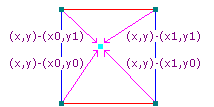
\includegraphics[height=\imgHeight]{images/noise_vectors.png}
    \caption{Vektoren von den Eckpunkten zu einem Punkt im Inneren einer Zelle im 2D}
    \label{fig:noise_vectors}
\end{figure}

Anschließend wird dann für jeden Eckpunkt
das Skalarprodukt aus dem dortigen Gradienten und dem Vektor in Richtung des Punktes gebildet. Der Mittelwert all dieser Skalarprodukte ergibt
dann den finalen Noise-Wert. \cite{16_perlin}\footnote{Erklärung in Anlehnung an https://mzucker.github.io/html/perlin-noise-math-faq.html}

TODO: Erklärung mathematisch beschreiben, Abbildungen erneuern/in eine Abbildung zusammenfassen

\section{L-Systeme}
Ein weiteres bekanntes Konzept ist das der L-Systeme.

\section{Fraktale}
\cite{19_mandelbrot_frame}




example-based model synthesis -> (weitere Merrell Verfahren) -> wave function collapse -> example-based procedural modeling using graph grammars